This section describes how ReDF models can be implemented in ASP. We do this for the basic problem of tiling, as well as for the purely relational data factorization presented before. Implementations of the other variations are included in Appendix \ref{ASP_appendix}. Our primary implementation is written in Clasp, can be used with the Clasp system \parencite{ASPbook,BrewkaCACM} and will be made available online upon acceptance of this manuscript.

\subsection{General computation methods: greedy and sampling approaches.} 
In all described problems, the goal is to find $k$ patterns or tiles, where a pattern is interpreted as a set of facts corresponding to a particular value of the latent variable. 
We will follow an iterative approach to finding these patterns,
in which the discovery of the next pattern or tile will be encoded in ASP.
We will consider both a {\em greedy} and a {\em sampling} algorithm
for realizing this. The sampling approach is intended for better scalability and will
be evaluated in Section \ref{subsec:experiments_tiling}.

\textit{Greedy model.}
The greedy approach is described  in  Algorithm \ref{alg:greedy}. Essentially, 
when the next best \tile has been computed (where \tile is a set of facts associated with the \tile identifier, e.g., in tiling a pattern is a set of transactions and attributes), it is added to the current set of \tiles. The specific part for each tile is represented by \texttt{executeProgram} and is encoded separately in ASP. Note that this greedy, iterative approach to finding $k$ patterns is very common in pattern mining. 
\changesb Theoretical bounds on the solution quality of the greedy approach have been studied in the context of the maximum $k$-set coverage problem \parencite{max_k_set_cover1, max_k_set_cover2}; more details can be found in Appendix \ref{appendix:k_set_coverage_analysis}. \changese
\begin{figure}[thb]
\captionof{algorithm}{Greedy execution model}
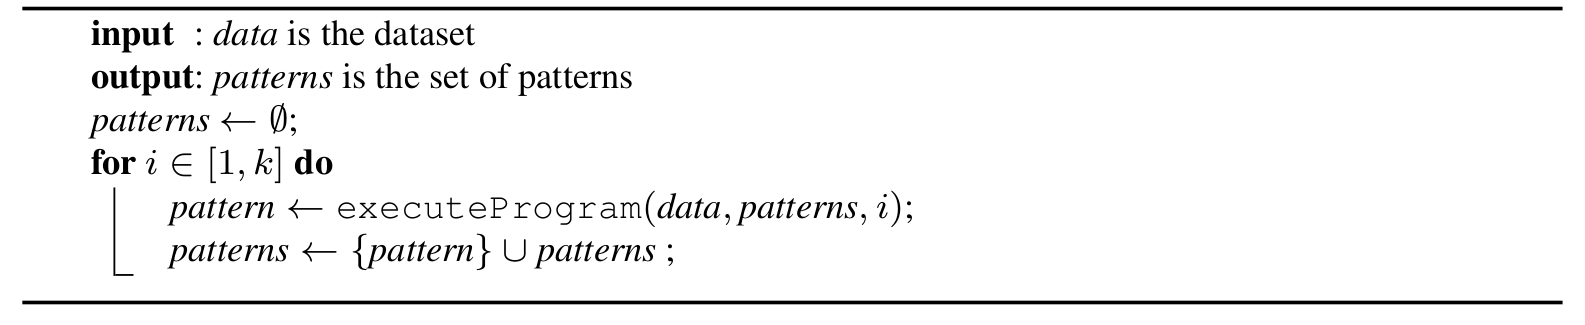
\includegraphics[width=\textwidth]{algorithm1_greedy.png}
 \label{alg:greedy}
\end{figure}

\textit{Column sampling execution model.} To improve scalability, we employ a sampling approach. Interestingly, our approach is different from most existing sampling techniques in data mining: instead of sampling a rows or patterns, we sample columns. Algorithm \ref{sampling} presents the column sampling approach we propose. The key difference with the greedy approach is that instead of determining the 
next best pattern on the {\em overall} dataset in each iteration, this approach samples $N$ subsets of the data
and determines the next best pattern for all of these subsets. The best among these is then fixed,
and the process is repeated. We empirically evaluate the effects of sampling
on the quality of the computed patterns and on the runtime in the experiment section. \changesb Quality bounds for this type of greedy search have also been analyzed previously \parencite{max_k_set_cover1}; for more details we refer to Appendix \ref{appendix:k_set_coverage_analysis}. \changese
\begin{figure}[thb]
\captionof{algorithm}{Column sampling execution model}
 \label{sampling}
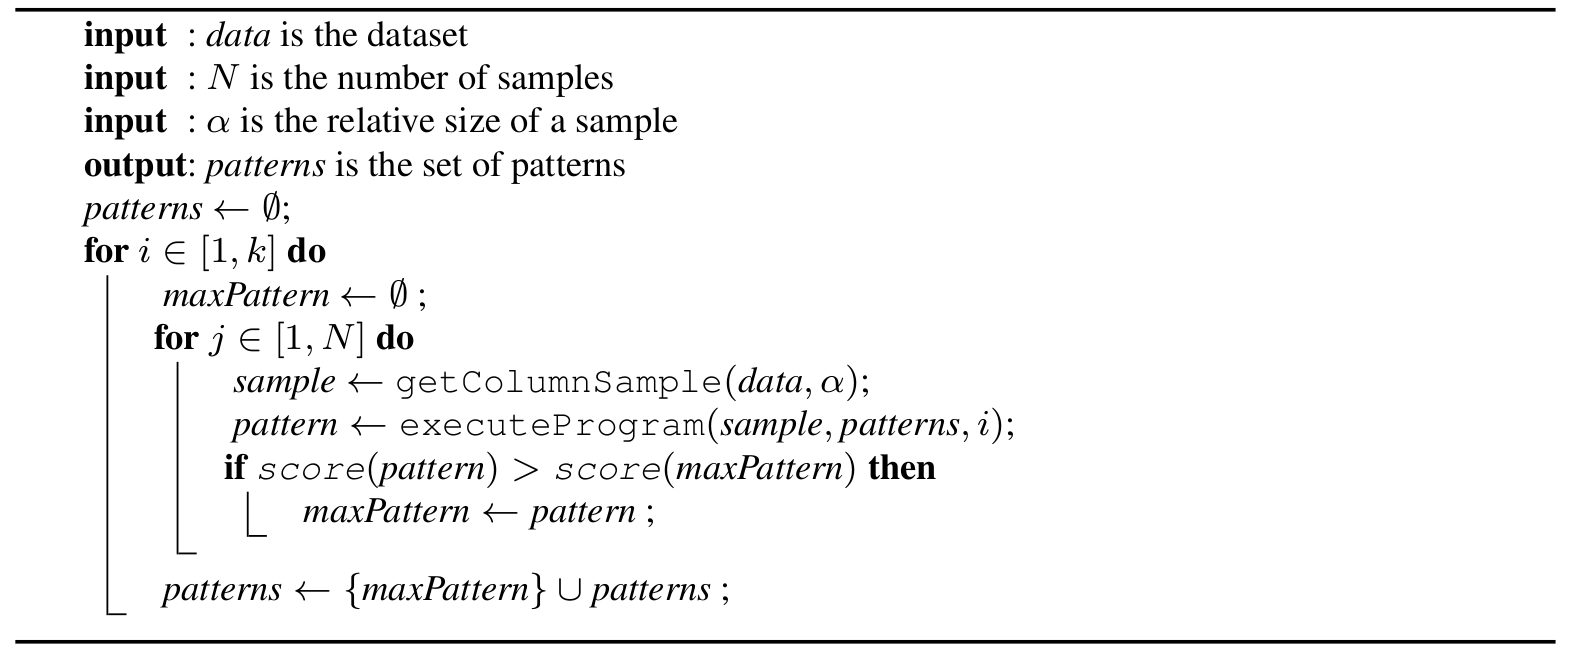
\includegraphics[width=\textwidth]{algorithm2_greedy_sampling.png}
\end{figure}

\lstset{numbers=left,
  numberstyle=\tiny,
  numbersep=5pt,
  basicstyle=\small,
  stringstyle=\sffamily,
  columns=fullflexible,
  flexiblecolumns=true,
  belowskip=5pt,
  alsoletter={-}, 
  alsodigit={:},
%  otherkeywords={},
  emph={%
      not,
      :-,
          },emphstyle={\bfseries}%
}
\begin{lstlisting}[float,floatplacement=t, caption=Greedy maximum $k$-tiling formalization in answer set programming, label=lst:encoding, escapeinside={@}{@}] 
@\commenttextasp{\%\onevalueConstraint; it generates at most one value per attribute}@
0 { tile(current, Value, Attribute) : valid(Attribute, Value) } 1 :- col(Attribute). @\label{guess_line}@
@\commenttextasp{\%\overcoverageConstraint}@
over_covered(current,T) :- not db(Val, Attr, T), tile(current, Val, Attr), transaction(T). @\label{overcover_line}@
@\commenttextasp{\%\intersectionConstraint}@
intersect(T) :- current != I, tile(current, Val, Attr), tile(I, Val, Attr), in(I,T). @\label{intersect_line}@
@\commenttextasp{\%defines presence of tiles in transactions}@
in(current,T) :- transaction(T), not over_covered(current, T), not intersect(T). @\label{in_line}@
@\commenttextasp{\%defines \maxcover function}@
covered(Transct, Attribute) :- in(Index,Transct), tile(Index, _, Attribute). @\label{covered_line}@
#maximize[covered(Transct, Attribute)]. @\label{maximize_line}@
\end{lstlisting}

\subsection{Data mining problems expressed in the framework} 

The maximum $k$-tiling problem can be encoded in answer set programming as indicated in Listing~\ref{lst:encoding}. The code implements the greedy model, i.e., Algorithm \ref{alg:greedy}, for the maximum $k$-tiling problem with a fixed number of tiles \parencite{tiling}. It assumes we have already found an optimal tiling for $n-1$ tiles, and indicates how to find the $n$-th tile to cover the largest area. The $n$-th tile is called \guess in the listing. \changesb Further, we have information about the names of the attributes and the possible values for each attribute through predicates $\col(\column)$ and $\valid(\column, \letter)$. That is, $\col(A)$ is an unary predicate that encodes possible column indices, and $\valid(A,V)$ is a binary predicate that encodes which possible values $V$ can occur in column $A$. \changese

Let us explain the code in Listing \ref{lst:encoding}. The constraint in Line \ref{guess_line} generates at most one value for each attribute. The constraints in Lines \ref{overcover_line} and \ref{intersect_line} compute the transactions where the current tile cannot occur, i.e., \texttt{intersect(T)} is the set of all transactions where the current tile overlaps with another tile and the current tile cannot cover these transactions. Similarly, \texttt{overcovered(currentI,T)} is the set of transactions that cannot be covered because there is an element in the current tile, with fixed index \texttt{currentI}, that is not present in transaction \texttt{T}. The constraint in Line \ref{in_line} states that if the tile does not violate the overcovering and intersection constraints in a transaction, it occurs in the transaction. Line \ref{covered_line} defines the coverage and the optimization constraint in Line \ref{maximize_line} enforces the selection of the best model.

\begin{theorem}[Correctness of the greedy ASP tiling encoding]\label{theorem:tiling}
 The ASP program \pprog defined by the Listing \ref{lst:encoding} computes the $k$-th largest tile w.r.t. the scoring function \maxcover (\ref{eqn:coverage-opt}) as extensions of the predicates $\code(k,\cdot,\cdot)$ and $\inrel(k,\cdot)$ in its answer set \as, provided that 
the dataset is represented extensionally through the predicates \db, \valid, and \col 
and the $k-1$ already found tiles are represented extensionally through the predicates $\code(I,\cdot,\cdot)$ and $\inrel(I,\cdot)$ for $I \in [1,k-1]$.
\end{theorem}
For the proof, see Appendix \ref{proof:tiling}.
The Clasp encodings for the other models are sketched in Appendix \ref{ASP_appendix}.

\subsection{Purely relational data factorization}
In Section \ref{sec:pure_decomposition} we presented a factorization of the \emph{publishedIn} relation into three binary relations. It constitutes a proof-of-concept prototype model in ASP and could be improved by, e.g., incorporating heuristics. %The proof of correctness is presented in Appendix \ref{sec:proof_pure_encoding}.
%\ref{lst:pure_alternative}

The general structure of the ASP encoding is similar to the \emph{sells} example in Listing \ref{lst:sells}: we indicate here only a possible optimization for the relation generators.  We use the left-to-right order of the atoms in the schema (replicated below) while generating candidates for the factorization.

% @\commenttextasp{\%factorization shape}@
% approx(A,U,V)      :- works_at(A,U), publishes_at(A,V), known_at(U,V). @\label{lst:pure:line:approx}@
% @\commenttextasp{\%relation generators}@
% @\commenttextasp{\%optimization function}@
% incorrect(A,U,V) :- approx(A,U,V), not p(A,U,V). @\label{lst:pure:incorrect1}@
% incorrect(A,U,V) :- not approx(A,U,V), p(A,U,V). @\label{lst:pure:incorrect2}@
% #minimize[incorrect(A,U,V)]. @\label{lst:pure:minimize}@
\begin{lstlisting}[caption=Generators for the model without a latent variable into three binary relations, escapeinside={@}{@}, label=lst:pure_alternative] 
0 { works_at(A,U)     } 1 :- published_in(A,U,V). @\label{lst:pure:gen1}@
0 { publishes_at(A,V) } 1 :- published_in(A,U,V), works_at(A,U). @\label{lst:pure:gen2}@
0 { known_at(U,V) } 1 :- published_in(A,U,V),works_at(A,U),publishes_at(A,V).@\label{lst:pure:gen3}@
\end{lstlisting}


\textit{Implementation differences.} When we generalize the factorization encoding with two relations to three relations, we observe a slight implementation difference between them. Factorization with the two relation shapes can be naturally implemented using the core ASP generate-and-test paradigm. Once we have guessed an extension for a certain value of the latent variable, we propagate it to the second relation and test against the constraints. This strategy is often deployed in specialized algorithms \parencite{tiling, dbp}.
For a multiple relation shape we guess an extension of one relation, then we constrain the possible values we generate for the second value (e.g., see Line \ref{lst:pure:gen2} in Listing \ref{lst:pure_alternative}). In general, we can search for one at a time using a greedy strategy (as in tiling). Theoretically, we can simultaneously search for values of a latent variable by replacing the fixed latent parameter by a variable and searching over the latent parameter as well. The work of \cite{tias_topk} provides evidence that this approach does not scale well, unless special propagators are introduced into the solver. This technique would allow extending the method to other shapes with more than three relations.
